\begin{figure}
  \begin{center}
    \begin{minipage}{0.495\linewidth}
      \includegraphics[width=\textwidth, trim=51mm 6mm 15mm 12mm, clip]{iras09_1.4zoom.eps}
    \end{minipage}
    \begin{minipage}{0.495\linewidth}
      \includegraphics[width=\textwidth, trim=51mm 6mm 15mm 12mm, clip]{iras09_4.8zoom.eps}
    \end{minipage}
    \caption{\vlba\ highest resolution 1.4 GHz ({\it{left}}) and 5.0
      GHz ({\it{right}}) images of the \irs\ nucleus. The color scale
      spans \srms\ to the peak intensity $000 ~\mrms$. The white
      contours trace emission at 3, 6, 9, 12, 15, 30, and 60
      \srms\ and the black ellipses are the beam sizes.}
    \label{fig:high}
  \end{center}
\end{figure}

\begin{figure}
  \begin{center}
    \begin{minipage}{\linewidth}
      \includegraphics*[width=\textwidth, trim=0mm 0mm 0mm 0mm, clip]{composite.eps}
      \caption{\vla\ 4.8 GHz image of the \irs\ nuclear region. The
        color scale spans \srms\ to the peak intensity $000
        ~\mrms$. The red contours trace 4.8 GHz emission at 3, 6, 9,
        12, 15, 30, and 60 \srms\ and the red ellipse is the
        \vla\ beam. The blue and green contours are $-3$, 3, 6, 9, and
        12 \srms\ 1.4 GHz and 5.0 GHz, respectively, emission from the
        low resolution \vlba\ images. The corresponding \vlba\ beams
        are shown using the same color scheme. The off-set between the
        nucleus in the \vla\ and \vlba\ images is within the
        positional uncertainty of the \vla\ observation.}
      \label{fig:comp}
    \end{minipage}
  \end{center}
\end{figure}

\begin{figure}
  \begin{center}
    \begin{minipage}{\linewidth}
      \includegraphics*[width=\textwidth, trim=22mm 0mm 35mm 15mm, clip]{beam.eps}
      \caption{Jet velocity ($\beta \equic v/c$) as a function of
        line-of-sight viewing angle. The solid curve is calculated
        from Equation \ref{eqn:beam} by assuming $k = 3$ and plugging
        in values for $\theta$




, the jet clumpiness. The shaded
        regions denote velocities and viewing angles for which the
        projected distance of jet knot 4 from the nucleus cannot be
        reproduced for travel times greater than 500 kyr or less than
        70 kyr.}
      \label{fig:beam}
    \end{minipage}
  \end{center}
\end{figure}

\begin{figure}
  \begin{center}
    \begin{minipage}{\linewidth}
      \includegraphics*[width=\textwidth, trim=0mm 0mm 0mm 0mm, clip]{iras09-ci-fan.eps}
      \caption{The 2D probability distribution of nuclear flux density
        as a function of frequency for an assumed continuous injection
        synchrotron model (see Section \ref{sec:XXX} for description
        of CI model). The color scale denotes probability and filled
        circles with errors bars are measured fluxes at 1.4, 5.0, 8.4,
        and 14.9 GHz.}
    \end{minipage}
    \label{fig:fan}
  \end{center}
\end{figure}

\begin{figure}
  \begin{center}
    \begin{minipage}{\linewidth}
      \includegraphics*[width=\textwidth, trim=27mm 5mm 35mm 10mm, clip]{tsyn_k.eps}
      \caption{Synchrotron age as a function of $k$, the ratio of
        non-radiating particle to relativistic electron energies, for
        several values of $\Phi$, the radiating particle population
        volume filling factor. Each curve is calculated using
        parameters from the CI model with the maximum likelihood. The
        horizontal dotted line marks the 70 kyr age lower limit
        determined from nuclear scattered UV properties by H99.}
      \label{fig:age}
    \end{minipage}
  \end{center}
\end{figure}

%% \begin{figure}
%%   \begin{center}
%%     \begin{minipage}{0.5\linewidth}
%%       \includegraphics*[width=\textwidth, trim=66mm 25mm 70mm 18mm, clip]{eex.ps}
%%     \end{minipage}
%%     \caption{Zoom-in of EEx overlaid with contours for 1.4 GHz radio
%%       emission (green) and \hst\ imaged optical emission (blue). The
%%       red wedge marks the extent of scattered UV emission (see H99 for
%%       discussion). See the electronic edition of the Journal for a color
%%       version of this figure}
%%     \label{fig:eex}
%%   \end{center}
%% \end{figure}

%%%%%%%%%%%
% Defunct %
%%%%%%%%%%%
%%
%% \begin{overpic}{iras09_1.4field.eps}
%%   \put(21.5,34){
%%     \includegraphics[scale=0.5, %
%%       trim=50.5mm 13mm 19mm 15mm, clip]{iras09_1.4zoom.eps}
%%   }
%% \end{overpic}
